\documentclass[12pt,letterpaper]{article}
\usepackage[letterpaper,margin=1in]{geometry}
\usepackage{setspace}
\usepackage{graphicx}
\usepackage{booktabs}
\usepackage{amsmath}
\usepackage{cite}
\usepackage{caption}
\usepackage{array}
\usepackage{hyperref}

\hypersetup{hidelinks}
\setstretch{1.65}
\captionsetup{font=small}
\graphicspath{{figures/}}
\pagestyle{plain}

\title{\bfseries SGTONet: Boundary-Constrained Rare-Fault Triggering for Short-Horizon Hoister Fault-State Prediction}
\author{}
\date{}

\begin{document}
\maketitle
\vspace{-3em}

\noindent\textbf{Abstract---}
Reliable hoister monitoring requires anticipating a degradation state before an overspeed fault is fully developed, yet the most safety-relevant transition samples are scarce. In our hoister dataset, the second-level degradation state accounts for only 185 of 37,417 timestamps, and strong time-series classifiers can obtain high accuracy while never detecting it. We propose SGTONet, a state-graph trigger-oriented network for one-step fault-state prediction. A patch Transformer encoder captures local temporal changes; a state-transition graph constrains physically plausible evolution; a conservative classifier handles common states; and a boundary-gated rare-fault trigger selectively overrides the classifier only near valid precursor transitions. On 27 files and three file-level splits, SGTONet recovers class 9 with F1 0.5556, whereas DLinear, TimesNet, iTransformer, PatchTST, and a conservative SGTO baseline all score 0.0000. Ablations confirm the value of boundary gating, rare-context attention, and calibrated triggering.

\noindent\textbf{Keywords---} hoisting system, overspeed fault, future-state classification, rare fault prediction, industrial time series.

\section{Introduction}

Industrial hoisting systems are safety-critical assets, and overspeed degradation should be recognized before the fault state becomes unrecoverable. This digest studies a fixed-horizon future-state classification setting: given a current multivariate sensor window, predict the state label one step ahead. The task is difficult because the critical second-level degradation state is extremely rare. In the studied dataset, class 9 has only 185 timestamps out of 37,417, so high overall accuracy can coexist with complete rare-state collapse.

This failure mode appears in strong time-series classifiers. As shown later, DLinear, TimesNet, iTransformer, PatchTST, and a conservative SGTO baseline all obtain zero class-9 F1 under the same file-level split protocol. The main objective is therefore not simply to maximize accuracy. It is to recover the rare degradation state while keeping common-state predictions controlled.

The contribution is SGTONet, a state-graph trigger-oriented network for short-horizon hoister state prediction. SGTONet separates conservative multiclass classification from a rare-fault trigger. The classifier is deliberately conservative because common states dominate the data and should not be destabilized by rare-class upweighting. The trigger is deliberately restrictive because class 9 should only be proposed near plausible transition boundaries. It can override the base classifier only when its rare score exceeds a calibrated threshold and the sample satisfies transition-boundary and precursor-state constraints. This design targets the boundary region where the future label changes before the full sensor window looks like the future state.

\section{Task and Method}

Let $x_t$ denote the multivariate sensor vector at time $t$. For a window length $L$, the input is $X_t=\{x_{t-L+1},\ldots,x_t\}$, and the target is the future label $y_{t+\Delta}$. The digest focuses on $\Delta=1$, with $L=96$ and a window step of 8. Labels are from the set $\{1,5,7,9,3\}$, representing stop, normal operation, first-level degradation, second-level degradation, and fault occurrence. The binary direct-fault indicator is dropped from the input to avoid leakage.

Fig.~\ref{fig:method_overview} summarizes SGTONet. The method combines four modules, each addressing a specific weakness of flat time-series classification. First, a patch Transformer encoder is used because local changes around overspeed transitions may be brief and can be diluted by whole-window averaging. Second, a state-transition graph represents prior knowledge about physically plausible state evolution, reducing arbitrary jumps between labels. Third, a conservative future-state classifier handles the common states, where stable predictions are more important than aggressive rare alarms. Fourth, a patch-attentive rare trigger searches for localized evidence of the second-level degradation state and is allowed to affect the final prediction only under boundary and precursor constraints.

At inference, the final decision follows
\[
\hat{y} =
\begin{cases}
9, & s_9 \ge \tau,\ b=1,\ y_t \in \{5,7\},\\
\hat{y}_{\mathrm{base}}, & \text{otherwise},
\end{cases}
\]
where $s_9$ is the rare score, $\tau$ is the calibrated threshold, $b$ is the boundary flag, and $y_t$ is the current state. This rule prevents the rare trigger from firing globally and makes the method different from using only a class-weighted loss or a larger backbone.

\begin{figure}[t]
    \centering
    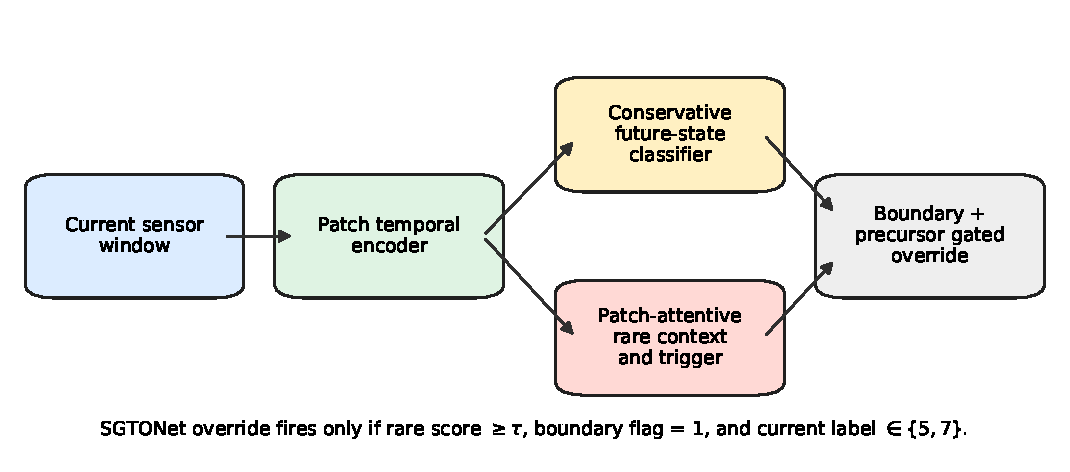
\includegraphics[width=0.95\linewidth]{fig0_method_overview.pdf}
    \caption{SGTONet decouples conservative future-state classification from a calibrated rare-fault trigger constrained by boundary and precursor semantics.}
    \label{fig:method_overview}
\end{figure}

\section{Experiments}

The dataset contains 27 files, 37,417 timestamps sampled every 4 seconds, and five state labels. The class counts are 10,959 for stop, 15,695 for normal operation, 5,364 for first-level degradation, 185 for second-level degradation, and 5,214 for fault occurrence. Evaluation uses file-level train/validation/test splits with split seeds 14, 22, and 30. The primary metrics are macro-F1, balanced accuracy, fault macro-F1, and class-9 precision/recall/F1.

\begin{table}[t]
\centering
\caption{Main comparison on the $\Delta=1$ future-state classification task. Values are three-split means.}
\label{tab:main}
\begin{tabular}{lrrrr}
\toprule
Method & Acc. & Macro-F1 & Fault F1 & C9 F1 \\
\midrule
SGTONet & 0.7102 & 0.6233 & 0.5411 & 0.5556 \\
iTransformer & 0.8175 & 0.6185 & 0.4615 & 0.0000 \\
DLinear & 0.7895 & 0.5961 & 0.4426 & 0.0000 \\
TimesNet & 0.7958 & 0.5893 & 0.4275 & 0.0000 \\
PatchTST & 0.7559 & 0.5687 & 0.4194 & 0.0000 \\
SGTONetV4 & 0.7630 & 0.5605 & 0.3999 & 0.0000 \\
\bottomrule
\end{tabular}
\end{table}

Table~\ref{tab:main} shows that SGTONet has the best macro-F1 and fault macro-F1 among the tested models, but not the best accuracy. This is expected: the method is optimized for rare-fault recovery rather than top-line accuracy. iTransformer has the highest accuracy, yet its class-9 F1 is zero. Fig.~\ref{fig:class9} isolates this rare-class behavior.

\begin{figure}[t]
    \centering
    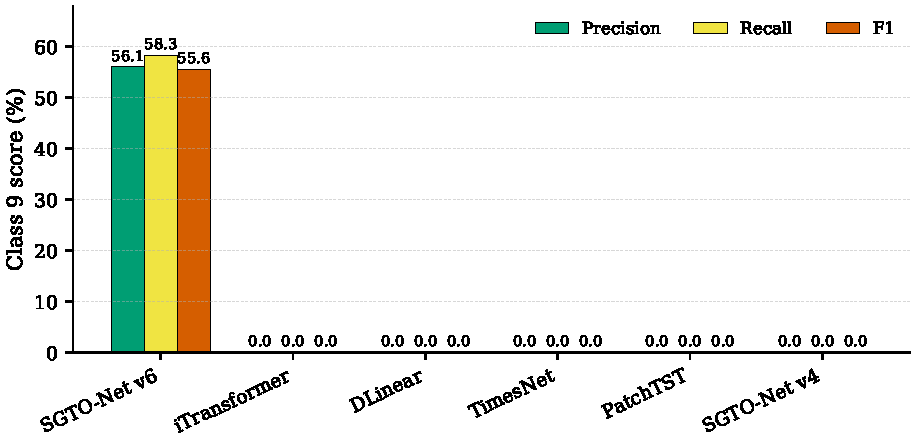
\includegraphics[width=0.90\linewidth]{fig2_class9_prf1.pdf}
    \caption{Class-9 precision, recall, and F1. Baselines collapse to zero class-9 F1, while SGTONet recovers the rare degradation state.}
    \label{fig:class9}
\end{figure}

\section{Ablation and Scope}

\begin{table}[t]
\centering
\caption{SGTONet ablation results on $\Delta=1$.}
\label{tab:ablation}
\begin{tabular}{lrrr}
\toprule
Variant & Macro-F1 & Bal. Acc. & C9 F1 \\
\midrule
Full SGTONet & 0.6233 & 0.6731 & 0.5556 \\
No precursor constraint & 0.6139 & 0.6725 & 0.5101 \\
Mean rare context & 0.5848 & 0.6654 & 0.2317 \\
No fallback prior & 0.5830 & 0.6397 & 0.3556 \\
No rare override & 0.5113 & 0.5568 & 0.0000 \\
No boundary constraint & 0.4550 & 0.5469 & 0.0158 \\
\bottomrule
\end{tabular}
\end{table}

Table~\ref{tab:ablation} supports the mechanism. Removing rare override collapses class-9 F1 to zero, which means the conservative base classifier alone does not solve rare-state recovery. Removing the boundary constraint causes uncontrolled triggering and reduces class-9 F1 to 0.0158. Replacing patch-attentive rare context with mean context also weakens rare recovery, indicating that local evidence inside the window matters.

\begin{figure}[t]
    \centering
    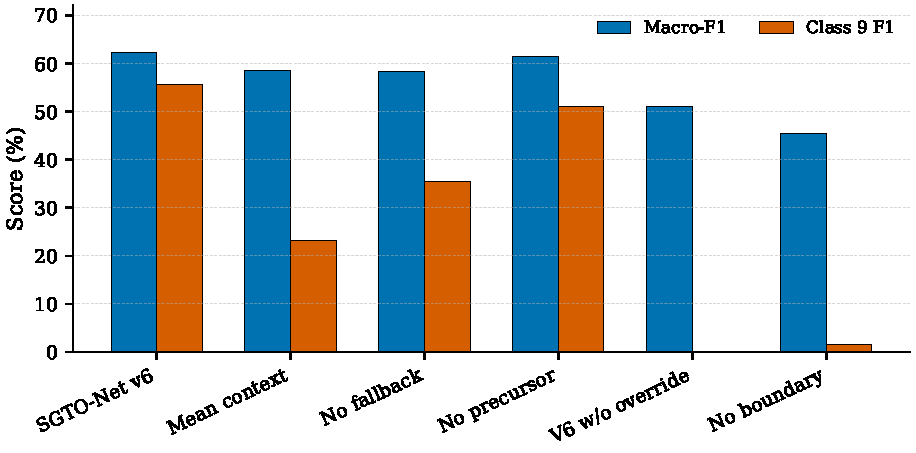
\includegraphics[width=0.90\linewidth]{fig3_ablation.pdf}
    \caption{Ablation study. Rare override, boundary constraint, fallback thresholding, and patch-attentive context all contribute to rare-fault recovery.}
    \label{fig:ablation}
\end{figure}

The current result should be scoped carefully. At $\Delta=3$, PatchTST reaches macro-F1 0.5877 and class-9 F1 0.1919, while SGTONet reaches macro-F1 0.5006 and class-9 F1 0.1070. Thus, the current configuration supports short-horizon rare-fault recovery, not general multi-horizon superiority.

\section{Conclusions and Future Works}

This digest identifies rare-boundary collapse as a practical failure mode in short-horizon hoister fault-state prediction. SGTONet addresses it by combining conservative multiclass prediction with a boundary-constrained rare-fault trigger. On the studied industrial dataset, the method recovers class 9 with F1 0.5556 while tested baselines obtain zero class-9 F1. Future work will validate the method on additional industrial assets, improve horizon-specific trigger calibration, and evaluate deployment-level false-alarm costs.

\begin{thebibliography}{9}
\bibitem{timesnet}
H. Wu, T. Hu, Y. Liu, H. Zhou, J. Wang, and M. Long, ``TimesNet: Temporal 2D-variation modeling for general time series analysis,'' in \emph{Proc. ICLR}, 2023.

\bibitem{itransformer}
Y. Liu, T. Hu, H. Zhang, H. Wu, S. Wang, L. Ma, and M. Long, ``iTransformer: Inverted transformers are effective for time series forecasting,'' in \emph{Proc. ICLR}, 2024.

\bibitem{patchtst}
Y. Nie, N. H. Nguyen, P. Sinthong, and J. Kalagnanam, ``A time series is worth 64 words: Long-term forecasting with transformers,'' in \emph{Proc. ICLR}, 2023.

\bibitem{dlinear}
A. Zeng, M. Chen, L. Zhang, and Q. Xu, ``Are transformers effective for time series forecasting?'' in \emph{Proc. AAAI}, 2023.
\end{thebibliography}

\end{document}
